\section{Reproducibility and provenance}
\label{app:provenance}
\subsection{Frozen final identities and audit boundary}
The final protocol is stored in \path{cja_en/review/changeos_p6_final_protocol_20260915.json}. It records full SHA-256 values for the final task set, a review report, the frozen three-event manifest, ChangeOS weights, source fingerprint, system prompt, policy configuration, and analysis scripts. Its own SHA-256 begins \texttt{41ccbb5fed5e}; exact paths and full hashes are retained in the machine-readable protocol rather than truncated in the audit. These identities describe the local execution; they are not substitutes for a publicly recoverable image and checkpoint package.

The dual-review procedure described in Section~\ref{sec:benchmark} requires two independent review records and an adjudication record linked to the frozen question identifiers. The available protocol lists one review-report path and hash; it does not separately identify those three records. Their inclusion and explicit mapping to the frozen set remain requirements for a complete release. This distinction prevents the execution audit from being interpreted as independent verification of the human-review process. Review records are provenance, not model inputs.

The 12 final shard directories contain manifests, preflight receipts, \path{episodes.jsonl}, \path{results.json}, and strict per-shard audits. Their combined report is \path{p6_final_three_event_v1_20260915_report.json} under \path{runs/benchmarks/changeos_binary/}; its SHA-256 begins \texttt{9e4370325bc9}. It validates 3,360 rows with zero execution errors, exact question/configuration/repeat coverage, and declared input identities. This is a local execution and consistency audit, not an independent re-execution of the full model pipeline. The run uses a fixed ChangeOS checkpoint and a locally loaded Qwen2.5-VL-7B-Instruct model; checkpoint identity and generation settings must accompany any release rather than be inferred from an online model name.

Scene construction and rendering are in the \path{backend/} modules \path{world.py}, \path{geo.py}, \path{xbd_map.py}, \path{fov_ladder.py}, and \path{perception.py}. Inspection, reobservation, and local Qwen calls are in the same directory's \path{agent_vqa.py}, \path{recheck.py}, and \path{local_qwen_vl.py}. The headless protocol is under \path{scripts/benchmarks/}; this directory also contains \path{build_roi_index.py}, \path{gen_agent_vqa_testset_v2.py}, and \path{review_agent_vqa_testset.py} for coverage indexing, task generation, and review checks. The operator interface is under \path{frontend/src/}. This file map establishes software correspondence, not that every optional module was active in each policy.

The final cost audits are \path{runs/benchmarks/changeos_binary/p7_cost_observability_final_repeat0_20260917/report.json}, with corresponding repeat1 and repeat2 paths. The existing auditor was applied to four shards at a time because its duplicate key is not repeat-aware. Together the three reports cover 3,360 episodes and flag 42 incomplete terminal-motion traces. All logged recheck request, inferred allocation, execution, and episode totals agree. Search-action allocation details, component-level timing, actual flight time, and physical action mapping remain unavailable. A complete public reproduction package would additionally need the licensed source imagery, scene manifests and affine transforms, basemap availability, dependency lock, checkpoint retrieval instructions, and one replay with action/observation hashes.

\section{Historical diagnostics outside the main evidence chain}
\label{app:historical}
\subsection{Archived four-class camera and allocation study}
An earlier \texttt{xview2\_first} four-class pipeline evaluated 3,753 buildings in 44 ROIs. It is not the binary ChangeOS backend of the final study. Table~\ref{tab:fov} retains its camera-footprint results and Table~\ref{tab:allocation} its offline allocation at a 0.25 building-selection fraction. The old temperature, prediction-set threshold, four-class entropy normalization, and allocation scores are not used in the main experiment. These offline selections operate on paired stored predictions, not on executable closed-loop routes or question answers.

\begin{table}[htbp]
\centering\small
\caption{Historical four-class building-level camera diagnostic on the same 3,753 evaluation buildings. Not comparable to the binary ChangeOS final question endpoint.}
\label{tab:fov}
\input{tables/historical/xview2_first_fov}
\end{table}

\begin{table}[htbp]
\centering\footnotesize
\caption{Historical four-class offline allocation at a 0.25 building-selection fraction. The label-informed row uses evaluation labels and is not deployable.}
\label{tab:allocation}
\input{tables/historical/xview2_first_allocation}
\end{table}

\begin{figure}[htbp]
\centering
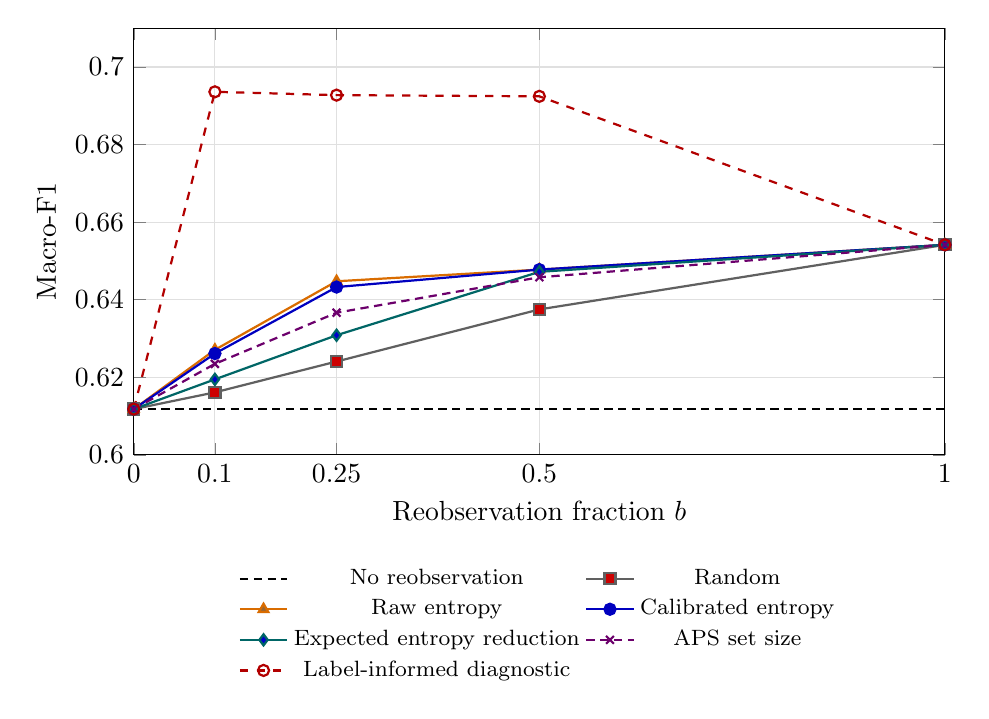
\begin{tikzpicture}
\begin{axis}[
  width=.98\linewidth,height=7.0cm,
  xlabel={Reobservation fraction $b$},ylabel={Macro-F1},
  xmin=0,xmax=1,ymin=.60,ymax=.71,
  xtick={0,.1,.25,.5,1},ytick={.60,.62,.64,.66,.68,.70},
  grid=major,grid style={black!12},
  legend style={at={(.5,-.24)},anchor=north,draw=none,font=\footnotesize},
  legend columns=2,
]
\addplot+[black,densely dashed,mark=none,thick] coordinates {(0,0.61180364) (0.1,0.61180364) (0.25,0.61180364) (0.5,0.61180364) (1,0.61180364)};
\addlegendentry{No reobservation}
\addplot+[gray!75!black,mark=square*,thick] coordinates {(0,0.61180364) (0.1,0.61611550) (0.25,0.62406965) (0.5,0.63750089) (1,0.65415042)};
\addlegendentry{Random}
\addplot+[orange!85!black,mark=triangle*,thick] coordinates {(0,0.61180364) (0.1,0.62708707) (0.25,0.64475982) (0.5,0.64776899) (1,0.65415042)};
\addlegendentry{Raw entropy}
\addplot+[blue!75!black,mark=*,thick] coordinates {(0,0.61180364) (0.1,0.62612436) (0.25,0.64326575) (0.5,0.64776853) (1,0.65415042)};
\addlegendentry{Calibrated entropy}
\addplot+[teal!80!black,mark=diamond*,thick] coordinates {(0,0.61180364) (0.1,0.61946892) (0.25,0.63084430) (0.5,0.64719004) (1,0.65415042)};
\addlegendentry{Expected entropy reduction}
\addplot+[violet!85!black,mark=x,thick] coordinates {(0,0.61180364) (0.1,0.62346363) (0.25,0.63665018) (0.5,0.64578998) (1,0.65415042)};
\addlegendentry{APS set size}
\addplot+[red!70!black,dashed,mark=o,thick] coordinates {(0,0.61180364) (0.1,0.69360303) (0.25,0.69275057) (0.5,0.69243946) (1,0.65415042)};
\addlegendentry{Label-informed diagnostic}
\end{axis}
\end{tikzpicture}

\caption{Historical offline four-class allocation sweep. Selected floor predictions replace cruise predictions; this is not a common-budget online policy curve.}
\label{fig:budget-curve}
\end{figure}

The archived matched-only sensitivity population contains 2,757 buildings detected at all three views (Table~\ref{tab:matched}). Because the subset is selected by detector success, it cannot replace the full 3,753-building endpoint. Its earlier exploratory ROI-bootstrap intervals, shown in Table~\ref{tab:cluster}, condition on fixed scores and the observed three events; they do not demonstrate transfer to new disasters.

\begin{table}[htbp]
\centering\small
\caption{Historical four-class matched-only sensitivity analysis.}
\label{tab:matched}
\begin{tabular}{lrrrr}
\toprule
View & Accuracy & Macro-F1 & Brier & NLL \\
\midrule
Cruise & 0.7918 & 0.7069 & 0.3367 & 0.6455 \\
Mid & 0.8052 & 0.7321 & 0.3176 & 0.6123 \\
Floor & 0.8099 & 0.7489 & 0.3175 & 0.6103 \\
\bottomrule
\end{tabular}

\end{table}

\begin{table}[htbp]
\centering\footnotesize
\caption{Historical four-class exploratory paired ROI-bootstrap differences at the 0.25 offline allocation fraction.}
\label{tab:cluster}
\begin{tabular}{lrr}
\toprule
Paired comparison & Macro-F1 difference & 95\% interval \\
\midrule
Calibrated entropy -- Random & +0.0192 & [+0.0097, +0.0419] \\
Calibrated entropy -- Raw entropy & -0.0015 & [-0.0093, +0.0061] \\
\bottomrule
\end{tabular}

\end{table}

\subsection{Archived VLN switch diagnostic}
The earlier 200-instruction VLN switch experiment used an earlier observation stack and one recorded run per configuration. Table~\ref{tab:vln-ablation} preserves the archived aggregate as a component diagnostic only. Enabling the recheck configuration did not cause recheck actions in that run; the table cannot establish a benefit from planning, memory, or reobservation under the current ChangeOS binary protocol.

\begin{table}[htbp]
\centering\footnotesize
\caption{Archived VLN switch diagnostic. SR is strict success within 25 m of the specified target; semSR accepts a matching damage-class building within 25 m. Recheck triggers were zero in all four configurations.}
\label{tab:vln-ablation}
\begin{tabularx}{\linewidth}{@{}l>{\raggedright\arraybackslash}Xrrrr@{}}
\toprule
Config. & Enabled navigation components & $n$ & SR (95\% CI) & semSR & NE (m) \\
\midrule
B0 & Keyword/greedy baseline & 200 & 0.070 [0.042, 0.114] & 0.165 & 222.3 \\
B1 & Hierarchical semantic planning & 200 & 0.080 [0.050, 0.126] & 0.155 & 223.9 \\
B2 & B1 + uncertainty recheck & 200 & 0.080 [0.050, 0.126] & 0.155 & 223.9 \\
B3 & B2 + topological memory & 200 & 0.080 [0.050, 0.126] & 0.140 & 305.7 \\
\bottomrule
\end{tabularx}

\end{table}
